En esta sección se comparará la implementación del filtro obtenida en la sección 3, que se denominará $H^{*}(s)$, con el filtro ideal $H(s)$

\subsection{Diagramas de Bode de módulo y fase}

\begin{figure}[!h]
    \centering
    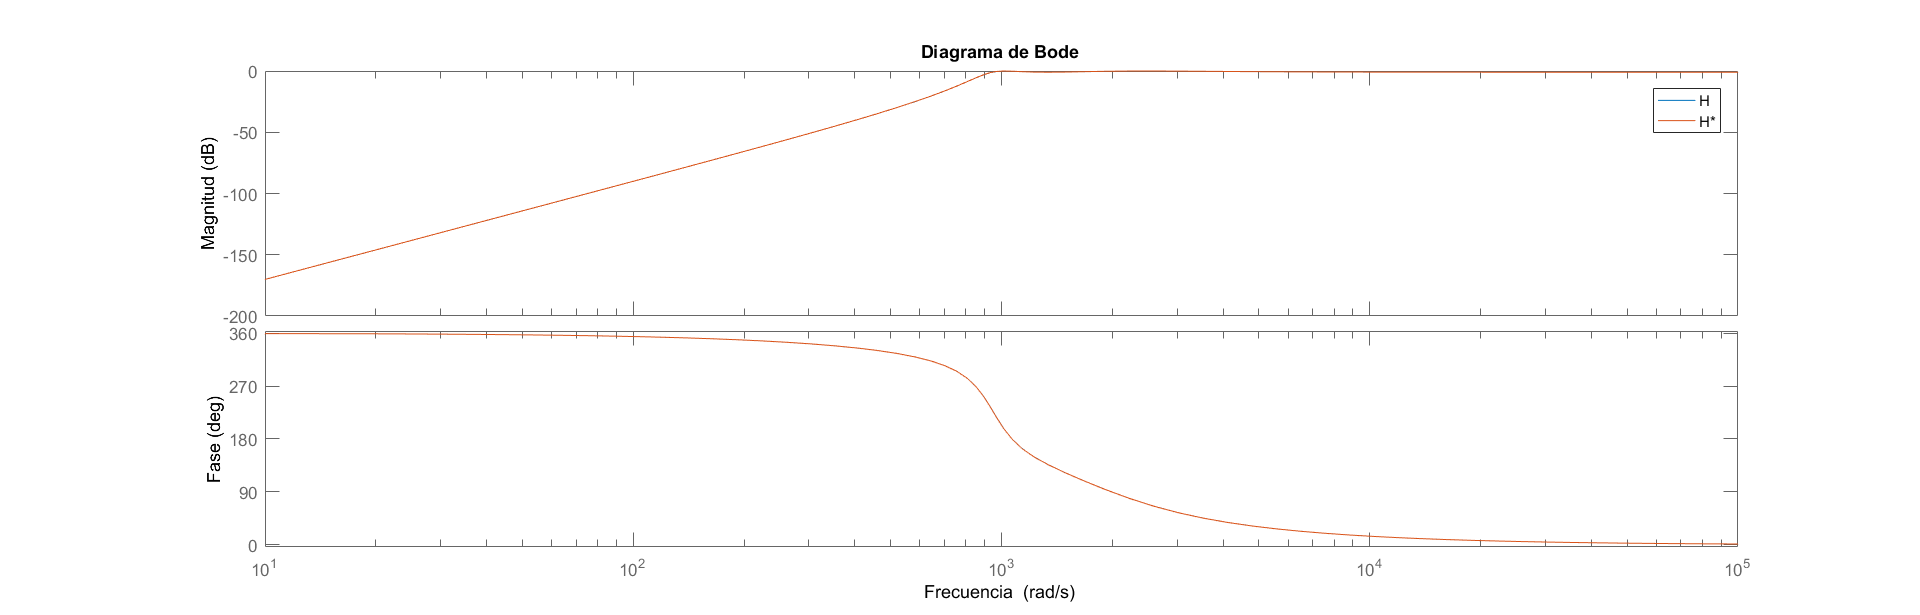
\includegraphics[width=1\textwidth]{resources/Comparacion_Bode.png}
    \caption{Comparación del diagrama de Bode}
\end{figure}

En este gráfico podemos ver que todo lo que ya fue mencionado previamente en el trabajo\\ práctico, el filtro es un pasaaltos pues para frecuencias menores a $\omega_0$ la señal se ve altamente atenuada y tendiendo a frecuencia 0 directamente se anula, mientras que para frecuencias mayores la señal se atenúa mucho menos y cuando se tiende a infinito la ganancia es constante.

\begin{figure}[!h]
    \centering
    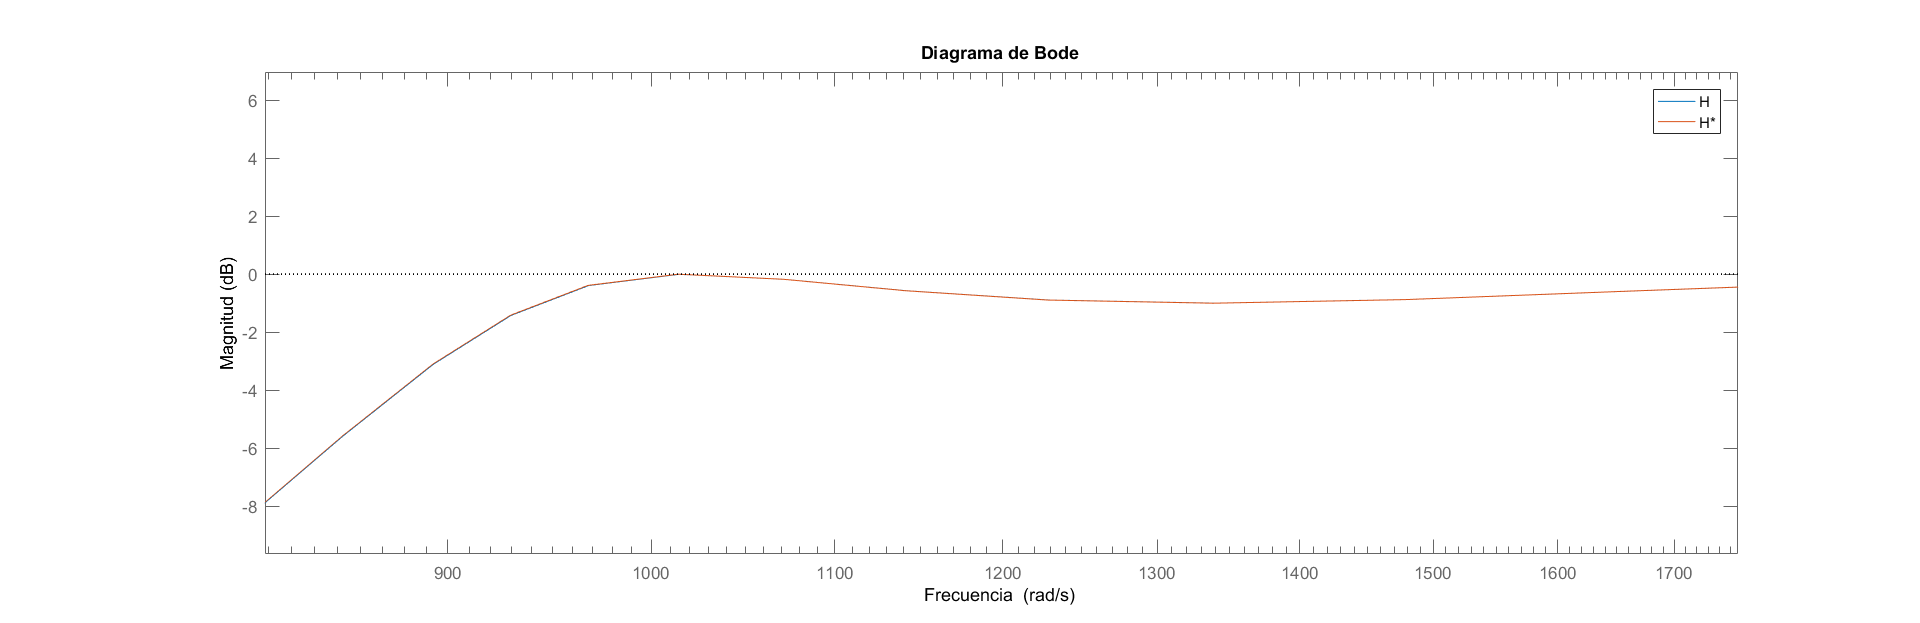
\includegraphics[width=1\textwidth]{resources/Bode_zoom.png}
    \caption{Pico en el diagrama de magnitud de Bode}
\end{figure}

En este gráfico podemos ver que efectivamente para $\omega_0 = 895 rad/s$ se alcanza $-3dB$ y luego para un valor cercano a este se alcanza un pico de $0dB$ aproximadamente en $1000 rad/s$.

Además, en este gráfico podemos ver que la diferencia entre el filtro implementado y el filtro ideal propuesto para el trabajo práctico es despreciable incluso a pequeñas escalas.

\subsection{Respuesta al escalón}
\begin{figure}[!h]
    \centering
    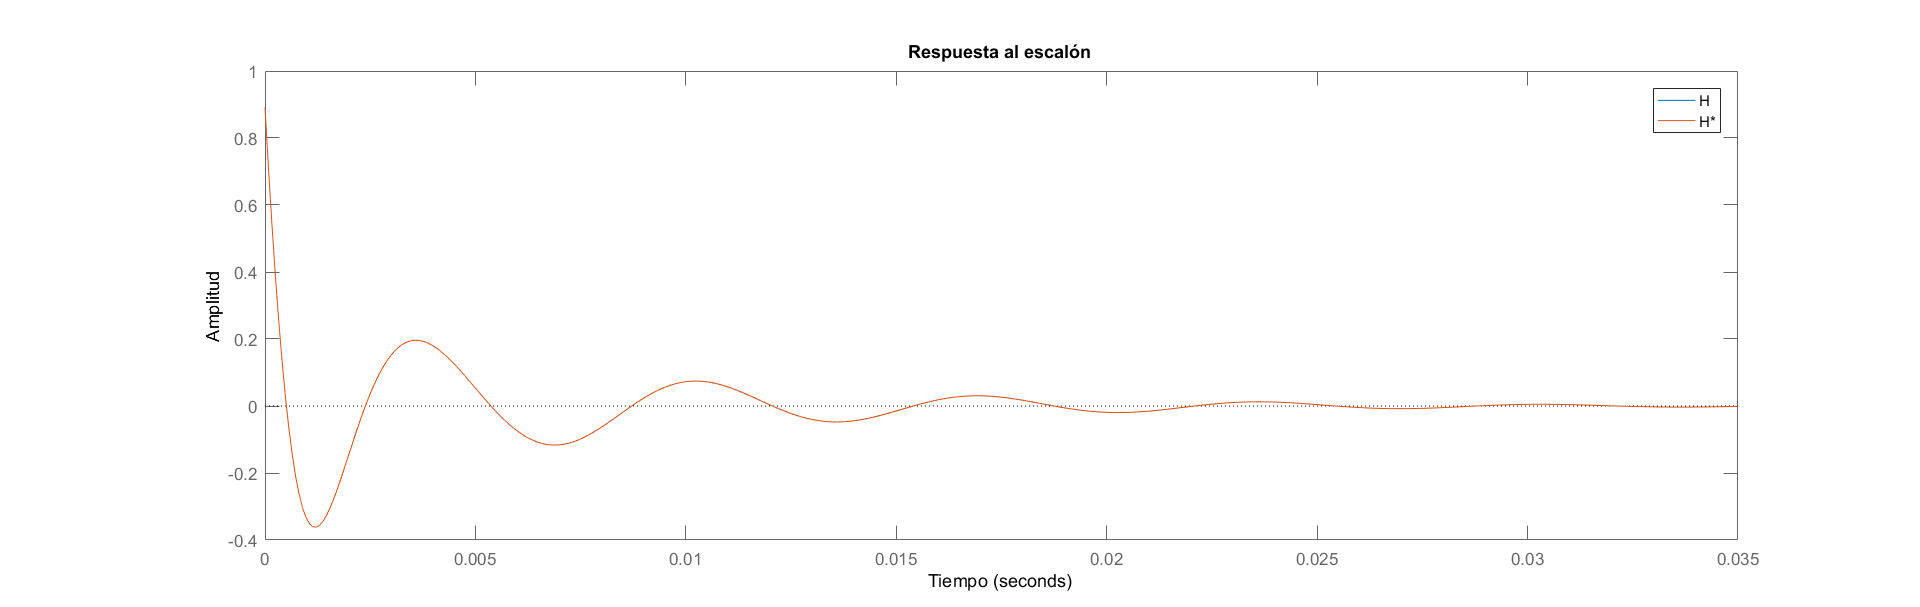
\includegraphics[width=1\textwidth]{resources/Comparacion_escalon.png}
    \caption{Comparación en respuesta al escalón}
\end{figure}

Teniendo en cuenta que la continua se trata de una señal de frecuencia cero, la señal tiende a anularse en la salida ya que como se vio en el gráfico de Bode la ganancia tiende a $-\infty$ para una frecuencia nula. La perturbación inicial se debe al comportamiento transitorio del circuito que no es tenido en cuenta para los diagramas de bode. Previamente en las secciones anteriores se había calculado, para la transferencia ideal, la respuesta analítica al escalón:

\begin{align*}
    v_o(t) & = 1.1692cos(1374.31t)e^{-1136.16t} - 0.6416sen(1374.31t)e^{-1136.16t}\\
           & + -0.2782cos(939.5t)e^{-133.34t} -0.094sen(939.5t)e^{-133.34t}
\end{align*}

De aquí obtenemos la información de los $\tau$ del circuito, estos vienen de los coeficientes que acompañan a la variable en los expontentes: $1136.16$ y $133.34$, por lo que cada coeficiente tiene asociado un $\tau_i$ respectivametente:
$$
    \tau_1 = \frac{1}{1136.16} s = 0.88ms
$$
$$
    \tau_2 = \frac{1}{133.34} s = 7.50ms
$$
Por lo que, teóricamente, el circuito estará en régimen transitorio durante $5 max(\tau_1, \tau_2) = 5 \cdot 7.50ms = 37.5ms$. Si bien dicho valor no aparece en el gráfico, se puede percibir que en un valor aproximado ($35ms$) la señal se ve atenuada por completo, que es lo que se espera en la respuesta debido a lo analizado previamente en los diagramas de Bode. 

Además agregar que como el filtro es un pasa altos podemos ver que la salida a $t=0$ es 1, y eso es porque las altas frecuencias del inicio del escalón no se ven anuladas.


\subsection{Respuesta al impulso}
\begin{figure}[H]
    \centering
    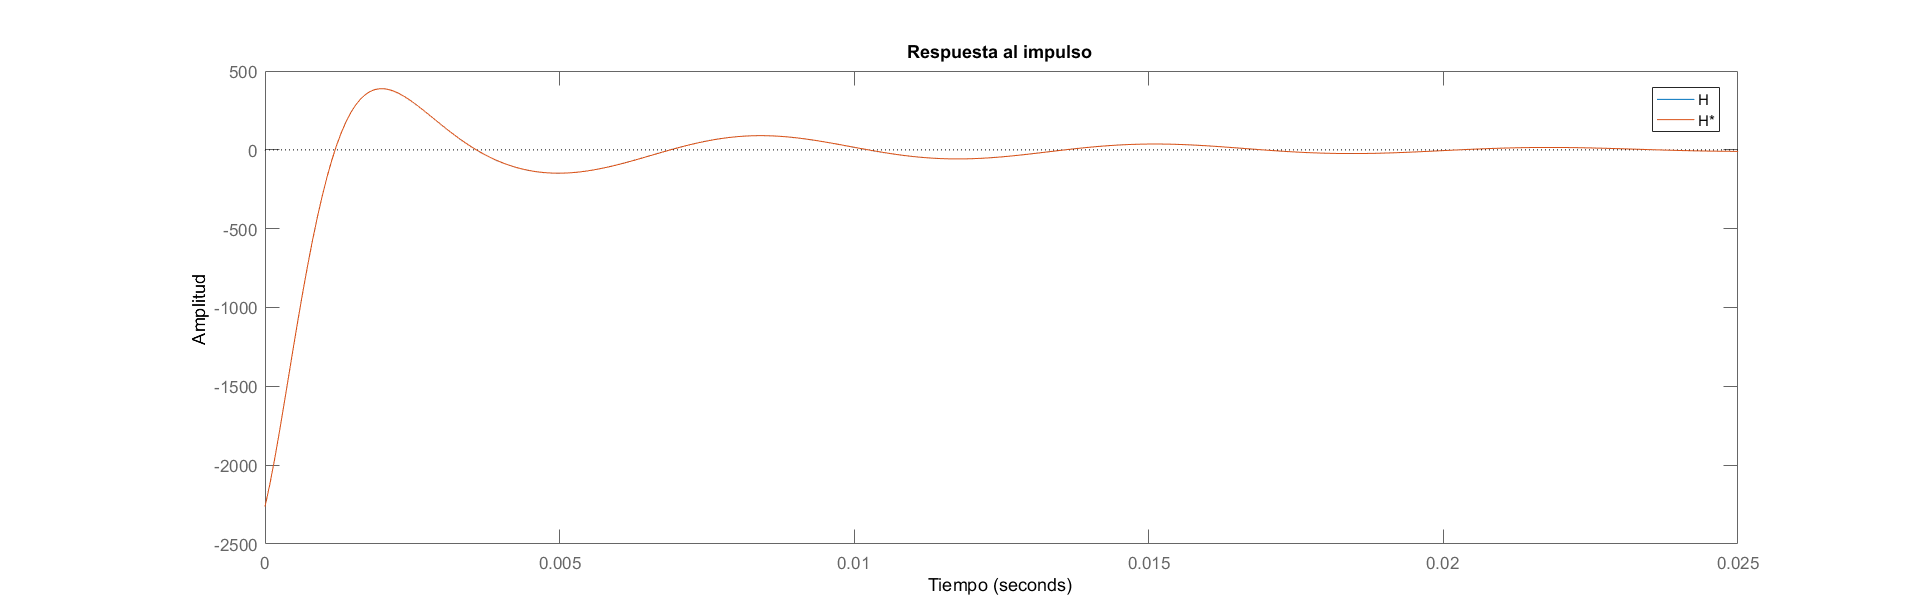
\includegraphics[width=1\textwidth]{resources/Comparacion_impulso.png}
    \caption{Comparación en respuesta al impulso}
\end{figure}
Podemos ver que, como en la respuesta al escalón, el $\tau$ es $37.5ms$, lo que se percibe en la el\\ gráfico. Prematuramente la señal alcanza valores muy negativos en la amplitud y luego crece rápidamente hasta un valor muy alto, cercano a 400 para luego tender a anularse para un tiempo cercano a $20ms$.

Como sabemos, el impulso corresponde a la derivada del escalón, y por ende se esperaba ver la misma relación entre las respuestas a ambas señales:

\begin{figure}[H]
    \centering
    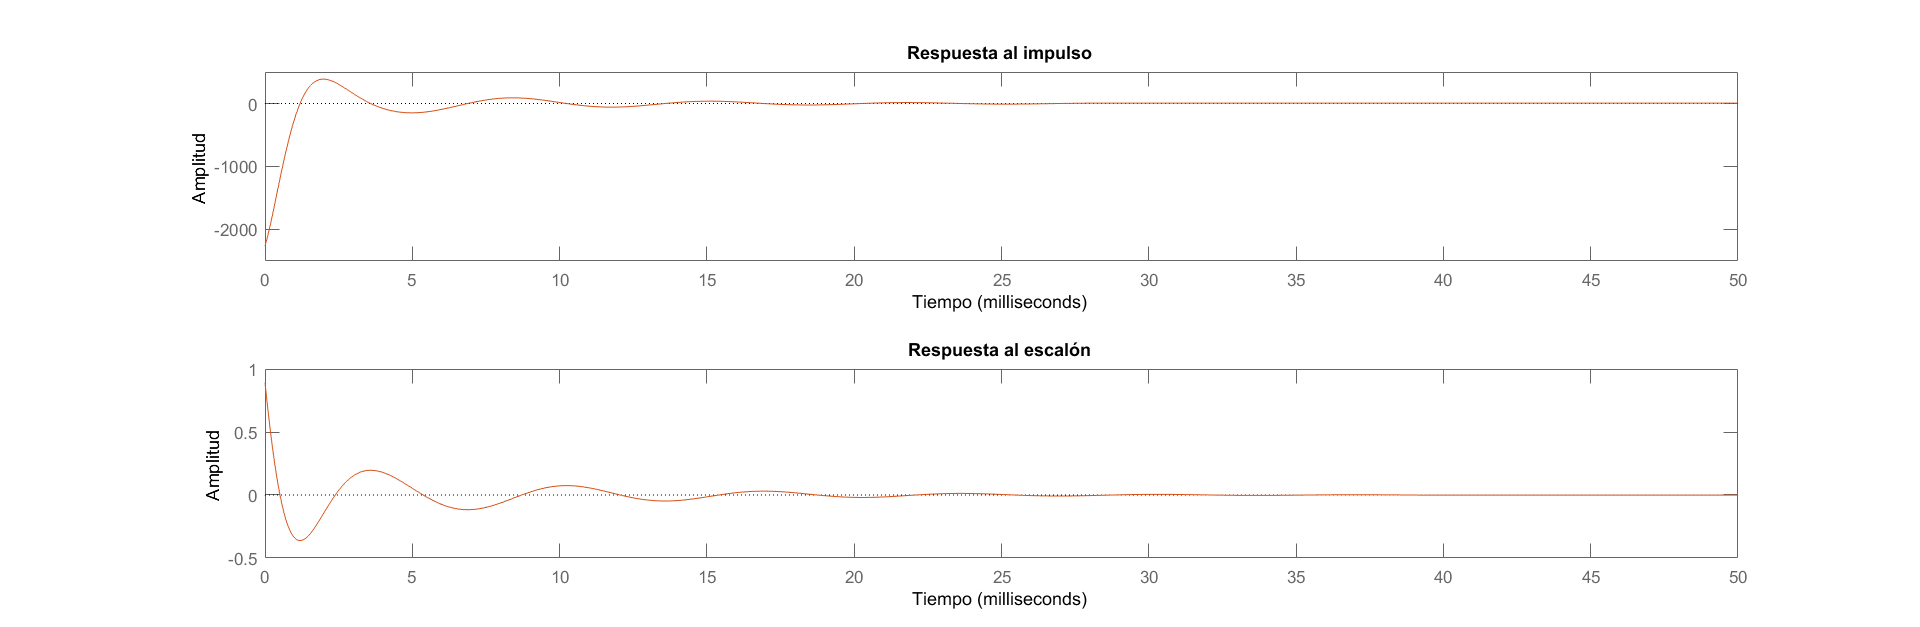
\includegraphics[width=1\textwidth]{resources/impulso_escalon.png}
    \caption{Comparación en respuesta al impulso}
\end{figure}

Comparando ambos gráficos se puede notar que cuando la respuesta al impulso se anula, la respuesta al escalón alcanza un máximo. Y además la magnitud de la respuesta al impulso se\\ puede asociar fácilmente a la tasa de cambio de la respuesta al escalón.

\subsection{Respuesta a señal senoidal}
Las frecuencias fueron elegidas para lograr entender el funcionamiento del filtro. Se escogió la frecuencia de corte de manera que se pueda ver que la señal se vea efectivamente atenuada $-3dB$ y que la fase sea aproximadamente $\pi rad$ como se vio en el diagrama de Bode. Luego se escogió $0.1 \cdot \omega_0$ para ver que la señal se vea completamente atenuada y $10 \cdot \omega_0$ para ver si la señal se atenúa aproximadamente un $10\%$ y la fase se deja intacta.

\begin{figure}[H]
    \centering
    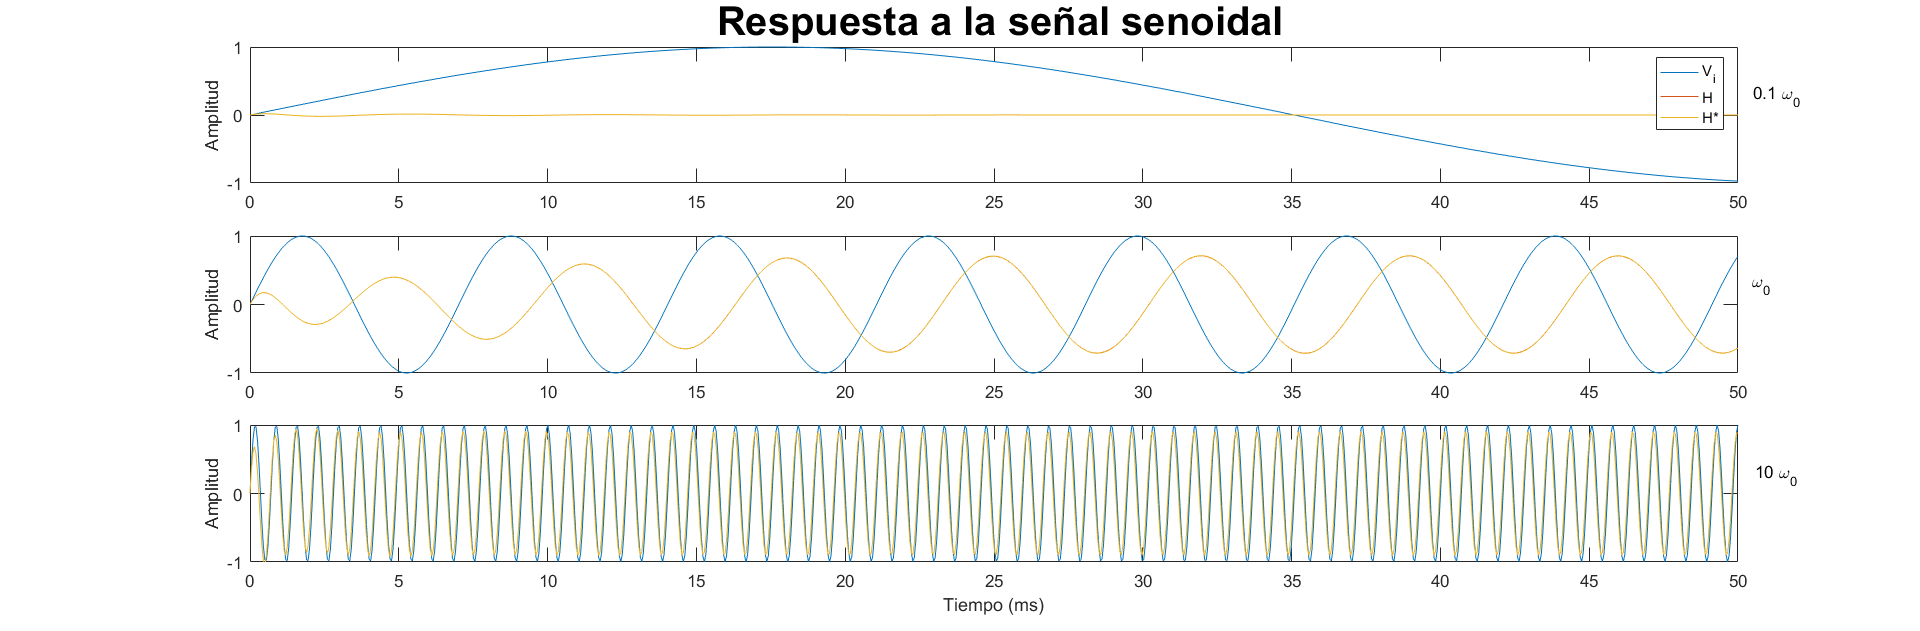
\includegraphics[width=1\textwidth]{resources/Comparacion_Seno.png}
    \caption{Comparación en respuesta a señal senoidal}
\end{figure}

Todas las premisas previamente mencionadas se vieron cumplidas en el gráfico. Podemos ver perfectamente que para el primer gráfico la señal se ve completamente atenuada, pues su frecuencia es 10 veces menor a la frecuencia de corte. Para la frecuencia de corte se puede ver que la respuesta se atenúo cerca del $30\%$ ($-3dB$) y se desfasó $\pi rad$. Luego, para 10 veces la frecuencia de corte se puede ver que la respuesta se encuentra en fase con la señal de entrada, y que además la atenuación es poca que coincide con el $10\%$ esperado.

\subsection{Respuesta a señal cuadrada}
\begin{figure}[H]
    \centering
    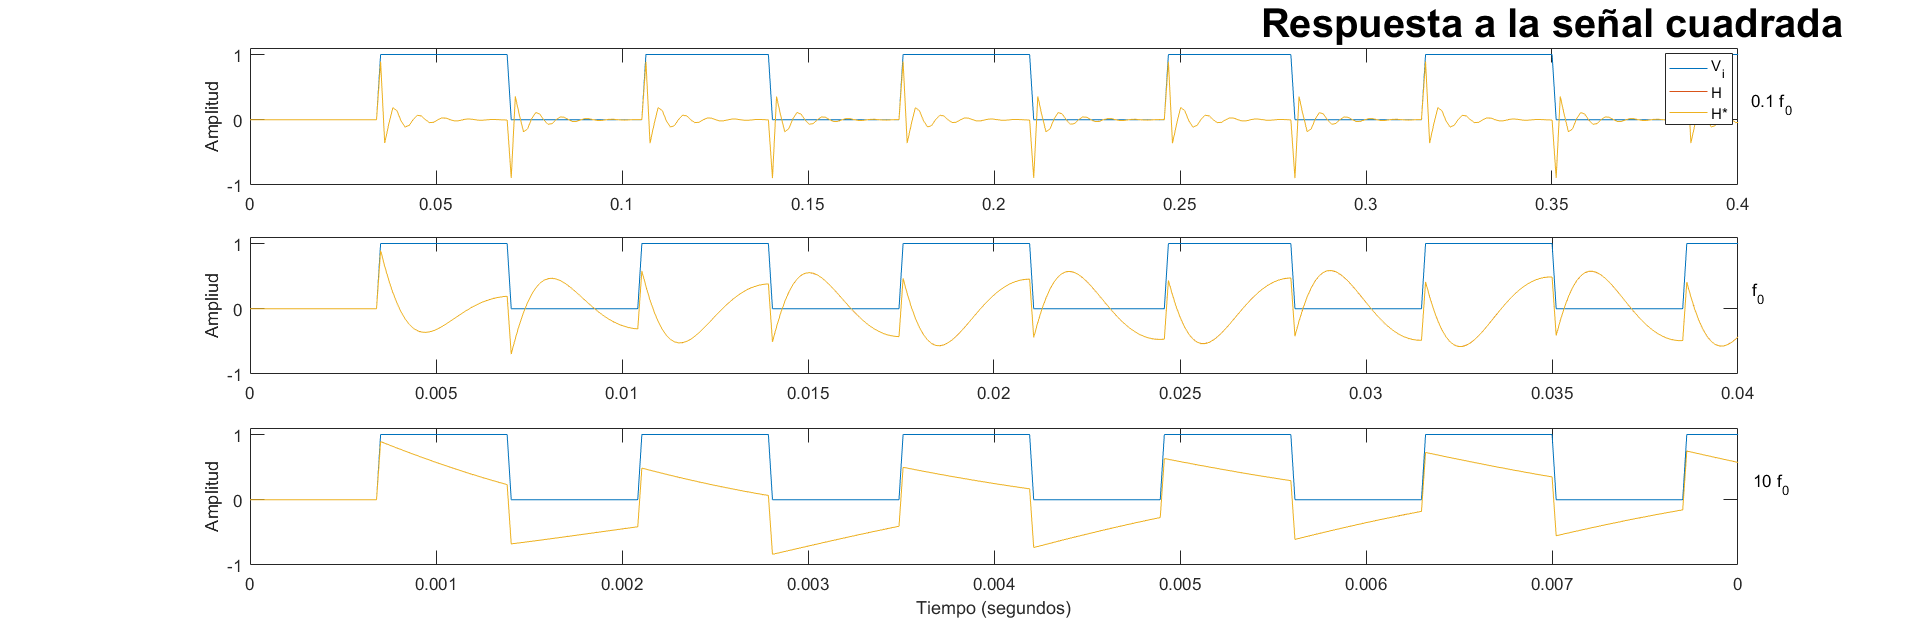
\includegraphics[width=1\textwidth]{resources/Comparacion_Cuadrada.png}
    \caption{Comparación en respuesta a señal cuadrada}
\end{figure}

Como ya se ha analizado la respuesta al escalón, es importante tenerla en cuenta para el análiis de la respuesta a la señal cuadrada, pues se trata de un tren de escalones. Hay que recordar que la respuesta al escalón tenía un $5 \cdot \tau \approx 37.5ms$.

Para el primer gráfico se puede observar que la señal está activa durante $35ms$, por lo que se puede observar que para cada activación la respuesta obtenida es similar a la del escalón.

Para el segundo gráfico la señal está activa durante $3.5ms$ por lo que no le da tiempo de atenuarse por completo, como se puede observar. Sin embargo podemos ver que la señal no se parece nada a la respuesta. Luego a medida que se va aumentando la frecuencia la señal comienza a parecerse a la señal de entrada, como ya se puede observar en el tercer gráfico donde la frecuencia es 10 veces la de corte.